% Authors: Nelson Lago and Fernanda Magano
% This file is distributed under the MIT Licence

%%%%%%%%%%%%%%%%%%%%%%%%%%%%%%%%%%%%%%%%%%%%%%%%%%%%%%%%%%%%%%%%%%%%%%%%%%%%%%%%
%%%%%%%%%%%%%%%%%%%%%%%%%%%%%%%%% PREÂMBULO %%%%%%%%%%%%%%%%%%%%%%%%%%%%%%%%%%%%
%%%%%%%%%%%%%%%%%%%%%%%%%%%%%%%%%%%%%%%%%%%%%%%%%%%%%%%%%%%%%%%%%%%%%%%%%%%%%%%%

% aspectratio default é 4:3;
% as mais úteis são 169 (16:9), 1610 (16:10) e 149 (14:9)
% A língua padrão é a última citada
\documentclass[xcolor={usenames,svgnames,dvipsnames},brazil,english,12pt,aspectratio=149]{beamer}

% Funções auxiliares essenciais
\usepackage{etoolbox}
\usepackage{xstring}
\usepackage{xparse}

% Vários pacotes e opções de configuração genéricos
\input{extras/basics}
% A fonte precisa ser definida depois que o tema metropolis foi carregado
%\input{extras/fonts}
\input{extras/floats}
% index não é necessário, mas deixamos aqui para usar os mesmos
% passos de compilação que a tese
\input{extras/index}
\input{extras/hyperlinks}
\input{extras/source-code}
\input{extras/utils}

% Diretório onde estão as figuras; com isso, não é preciso colocar o caminho
% completo em \includegraphics (e nem a extensão).
\graphicspath{{figuras/}}

% Comandos rápidos para mudar de língua:
% \en -> muda para o inglês
% \br -> muda para o português
% \texten{blah} -> o texto "blah" é em inglês
% \textbr{blah} -> o texto "blah" é em português
\babeltags{br = brazil, en = english}


%%%%%%%%%%%%%%%%%%%%%%%%%%%% APARÊNCIA DO BEAMER %%%%%%%%%%%%%%%%%%%%%%%%%%%%%%%

\usepackage{appendixnumberbeamer}

% Tema metropolis com algumas modificações
\dowithsubdir{extras/}{\usetheme{imeusp}}

% O padrão usa um tom de vermelho escuro como cor principal; a opção
% "greeny" troca essa cor por um tom de verde; a opção "sandy" usa o
% mesmo tom de verde mas modifica a cor padrão dos blocos para um
% tom amarelado.
\dowithsubdir{extras/}{\usecolortheme[greeny]{imeusp}}
% Desabilita a cor de rodapé
\setbeamercolor{footline}{fg=,bg=}

%%%%%%%%%%%%%%%%%%%%%%%%%% COMANDOS PARA O USUÁRIO %%%%%%%%%%%%%%%%%%%%%%%%%%%%%

\newcommand\col{\column{.5\textwidth}}

% A cada nova seção, recapitula o sumário
% Para desabilitar, é só comentar este trecho
\AtBeginSection[]{
  \begin{frame}<beamer>{Visão Geral}
    \intermezzo
  \end{frame}
}

% Blocos de cor personalizada
\newenvironment{coloredblock}[2]%
{
    \setbeamercolor{block title}{fg=white,bg=#1!80!white}
    \setbeamercolor{block body}{fg=darkgray,bg=#1!20!white}
    \setbeamercolor{local structure}{fg=darkgray,bg=#1!20!white}
    \begin{block}{#2}
}{
    \end{block}
}

%%%%%%%%%%%%%%%%%%%%%%%%%%%%%%%%% METADADOS %%%%%%%%%%%%%%%%%%%%%%%%%%%%%%%%%%%%

% Referências
\usepackage[style=bwl-FU]{biblatex}
\addbibresource{bibliografia.bib}
% Acrescenta à lista de referências sem precisar incluir uma referência
% de fato no texto
\nocite{bronevetsky02,schmidt03:MSc, FSF:GNU-GPL, CORBA:spec, MenaChalco08}
% Acrescenta tudo do arquivo .bib
%\nocite{*}

\title[The shortened title]{Experimentação baseada em Simulação em Sistemas para Cidades Inteligentes}
\subtitle{}

\author[Authors Name]{Lucas Kanashiro}

%\institute[USP]{\textbf{Workshop Name} \\ Computer Science Department \\ IME USP}
\institute[USP]{\textbf{Orientador: Prof. Dr. Fabio Kon} \\ Departamento de Ciência da Computação \\ IME USP}

\date{7 de Março de 2019}

% Coloca a imagem no fundo da página de título
\bgimage{\includegraphics[width=\paperwidth]{fundo_predios_e_grafo}}

% Logotipos no rodapé da página de título
\logos{
  \hfil\hfil\includegraphics[width=.1\textwidth]{usp-logo}\hfil%
  \raisebox{-.0103\paperheight}{\includegraphics[height=.0932\paperheight]{interscity-logo}}\hfil%
  \raisebox{-.033\paperheight}{\includegraphics[width=.07\textwidth,trim=0 230 0 0,clip]{ime-logo}}\hfil\hfil
}

%\logos{
%  \hfil\hfil\includegraphics[width=.1\textwidth]{usp-logo}\hfil%
%  \raisebox{-.0103\paperheight}{\includegraphics[height=.0932\paperheight]{interscity-logo}}\hfil%
%  \raisebox{-.00517\paperheight}{\includegraphics[height=.057\paperheight]{cnpq-logo}}\hfil%
%  \raisebox{-.0342\paperheight}{\includegraphics[height=.1035\paperheight]{capes-logo}}\hfil%
%  \includegraphics[height=.044\paperheight]{fapesp-logo}\hfil\hfil
%}

% Usado para criar o qrcode com o endereço da apresentação
%\presentationurl{http://interscity.org}

% Inclui o qrcode no sumário da apresentação
%\includeqrcodeintoc

% O slide de sumário pode ser dividido em colunas; o parâmetro
% determina após qual o número da seção fazer a quebra de coluna
% (use zero para uma coluna ou simplesmente omita este comando).
\toccolumns{8}


%%%%%%%%%%%%%%%%%%%%%%%%%%%%%%%%%%%%%%%%%%%%%%%%%%%%%%%%%%%%%%%%%%%%%%%%%%%%%%%%
%%%%%%%%%%%%%%%%%%%%%%%%%%%% INÍCIO DA APRESENTAÇÃO %%%%%%%%%%%%%%%%%%%%%%%%%%%%
%%%%%%%%%%%%%%%%%%%%%%%%%%%%%%%%%%%%%%%%%%%%%%%%%%%%%%%%%%%%%%%%%%%%%%%%%%%%%%%%

\begin{document}

% É complicado colocar uma imagem de fundo, os logos das agências e
% o conteúdo "normal" do slide de título sem que as coisas fiquem
% bagunçadas, então definimos um comando para gerar o slide de título
\customtitlepage

% Slide com o qrcode
%\showqrcode

\begin{frame}{Visão Geral}
  \overview
\end{frame}

\section{Introdução}

\begin{frame}[plain]
  \includegraphics[width=\textwidth]{chaotic_city.jpg}
  {\tiny Fonte: \href{https://www.flickr.com/photos/joiseyshowaa/2402764792/in/photolist-4EjNgb-4PMpwr-dseMM4-o2wJVc-cmJa3q-6mhvwX-9zDqmR-9BM7uJ-9zJBBx-fQetpQ-53jKRx-rbqw9A-F5tZZQ-bWMNF9-4bkrPW-ah98ef-4Do6tv-27JPj4G-Wp2dZ7-9RoTmJ-4hEZQo-zBRL-26Eg3uQ-5y1Bd1-aPujXi-61s8PT-7thSkH-753JxR-9pvEQ4-8VZKNS-b8EWyn-4XH2Zz-8vijrs-85Qjwh-fLoDcx-i8uvZ-s359a-GAoNUV-8A5qDY-ojAZeF-dreQ72-cegU7h-5Yka8U-2FRunS-dovsLg-yzxzG-TTJKuT-6xJa2s-doMGg7-65H6ko}{World Class Traffic Jam} / joiseyshowaa / \href{https://creativecommons.org/licenses/by-sa/2.0/}{CC BY-SA 2.0} }
\end{frame}

\begin{frame}[plain]
  \includegraphics[width=\textwidth]{smartcity2.jpg}
    %{\tiny Fonte: \url{http://realtyplusmag.com/wp-content/uploads/2017/07/smartcity.jpg} }
\end{frame}

\begin{frame}[standout]
	Como realizar experimentos nesses sistemas na escala de grandes cidades?!
\end{frame}

\section{Trabalhos Relacionados}

\begin{frame}{Trabalhos Relacionados}
    \begin{block}{Desafios em ambiente de experimentação para Cidades Inteligentes}
        \begin{itemize}
            \item Escala condizente com as cidades
            \item Heterogeneidade dos dispositivos de IoT
            \item Acesso concorrente aos diversos recursos da cidade
            \item Mobilidade dos recursos da cidade
            \item Reprodutibilidade desses ambientes
        \end{itemize}
    \end{block}
\end{frame}

\begin{frame}{Trabalhos Relacionados}
  \begin{block}{Implantação de Infraestrutura de IoT}
    \begin{itemize}
      \item Pequena escala
      \item Custo de aquisição, implantação e manutenção
      \item Menor flexibilidade
      \item Dificulta a reprodutibilidade
    \end{itemize}
  \end{block}
\end{frame}

\begin{frame}{Trabalhos Relacionados}
  \begin{block}{Uso de simulação}
    \begin{itemize}
      \item Simuladores de cidades inteligentes não são de larga escala
      \item Foco principal é simular diferentes topologias de rede
      \item Tentativa de representar mobilidade de recursos da cidade
      \item Não viabiliza execução de comandos de atuação
    \end{itemize}
  \end{block}
\end{frame}

\begin{frame}{Trabalhos Relacionados}
\begin{table}[htb!]
    \centering
    \resizebox{\textwidth}{!}{
\begin{tabular}{|c|c|c|c|c|c|l|}
\hline
    \thead{Ambiente de \\Experimentação}          & \thead{Uso de\\ dispositivos de IoT} & \thead{Uso de\\ simulação} & \thead{Implantação em \\ laboratório} & \thead{Implantação em \\ ambiente externo} & \thead{Larga\\ escala} & \multicolumn{1}{c|}{\thead{Execução de \\ comandos de atuação}} \\ \hline
\makecell{I3ASensorBed}                        & \textbf{x}                          & \textbf{x}                     & \textbf{x}                          & \textbf{x}                               & \textbf{}                     &                                                                       \\ \hline
\makecell{Padova Smart City}                   & \textbf{x}                          & \textbf{}                      & \textbf{}                           & \textbf{x}                               & \textbf{}                     &                                                                       \\ \hline
\makecell{FIT IoT-LAB}                         & \textbf{x}                          & \textbf{}                      & \textbf{}                           & \textbf{x}                               & \textbf{x}                    & \multicolumn{1}{c|}{\textbf{x}}                                       \\ \hline
\makecell{City of Things}                      & \textbf{x}                          & \textbf{x}                     & \textbf{}                           & \textbf{x}                               & \textbf{}                     &                                                                       \\ \hline
\makecell{Smart Berlin Testbed}                & \textbf{x}                          & \textbf{}                      & \textbf{}                           & \textbf{x}                               & \textbf{}                     &                                                                       \\ \hline
\makecell{SmartSantander}                      & \textbf{x}                          & \textbf{}                      & \textbf{}                           & \textbf{x}                               & \textbf{x}                    & \multicolumn{1}{c|}{\textbf{x}}                                       \\ \hline
\makecell{SmartCampus}                         & \textbf{x}                          & \textbf{}                      & \textbf{x}                          & \textbf{}                                & \textbf{}                     & \multicolumn{1}{c|}{\textbf{x}}                                       \\ \hline
\makecell{Birmingham Urban \\ Climate Laboratory} & \textbf{x}                          & \textbf{}                      & \textbf{}                           & \textbf{x}                               & \textbf{x}                    &                                                                       \\ \hline
\makecell{SmartGridLab}                        & \textbf{x}                          & \textbf{}                      & \textbf{x}                          & \textbf{}                                & \textbf{}                     &                                                                       \\ \hline
\makecell{Street Light Poles}                  & \textbf{x}                          & \multicolumn{1}{l|}{}          & \multicolumn{1}{l|}{}               & \textbf{x}                               & \multicolumn{1}{l|}{}         &                                                                       \\ \hline
\makecell{OpenMTC}                             & \textbf{x}                          & \multicolumn{1}{l|}{}          & \multicolumn{1}{l|}{}               & \textbf{x}                               & \textbf{x}                    &                                                                       \\ \hline
\makecell{CityBench}                           & \multicolumn{1}{l|}{}               & \multicolumn{1}{l|}{}          & \multicolumn{1}{l|}{}               & \multicolumn{1}{l|}{}                    & \textbf{x}                    &                                                                       \\ \hline
\end{tabular}
    }
    \caption{Caracterização dos trabalhos relacionados}
    \label{tab:trabalhos_relacionados}
\end{table}
\end{frame}

\begin{frame}[standout]
	Trabalhos ditos de larga escala não conseguem representar o contexto de grandes cidades!
\end{frame}

\section{Objetivo}

\begin{frame}
    \begin{block}{Objetivo Geral}
        Prover um mecanismo para construção de um \textbf{ambiente de experimentação} de \textbf{larga escala} e \textbf{interativo} para sistemas de Cidades Inteligentes através de \textbf{simulação}.
    \end{block}
\end{frame}

\begin{frame}{Objetivos}
    \begin{block}{Desafios}
        \begin{itemize}
            \item Definição de uma arquitetura de software para solução
            \item Implementação e análise de estudos de caso para validação da solução
                \begin{itemize}
                    \item InterSCSimulator
                    \item Plataforma InterSCity
                \end{itemize}
        \end{itemize}
    \end{block}
\end{frame}


\section{Proposta de Solução}

\begin{frame}{Requisitos}
    \begin{block}{Fundamentais}
        \begin{itemize}
            \item Modelos aderentes à realidade de uma cidade
            \item Tempo de execução igual ao tempo real
            \item Geração de grande massa de dados
            \item Comunicação em tempo de execução
        \end{itemize}
    \end{block}
\end{frame}

\begin{frame}{Requisitos}
    \begin{block}{Integração}
        \begin{itemize}
            \item Integração semântica
                \begin{itemize}
                    \item Recurso da cidade
                    \item Capacidades inerentes de cada recurso da cidade
                \end{itemize}
            \item Interoperabilidade de protocolos de comunicação
            \item Envio de dados de sensoriamento em tempo real
            \item Recebimento de dados de atuação em tempo real
        \end{itemize}
    \end{block}
\end{frame}

\begin{frame}[plain]
    \begin{center}
        \includegraphics[width=.4\textwidth]{integration-general-architecture.png}
    \end{center}
\end{frame}

\begin{frame}[plain]
    \begin{center}
        \includegraphics[width=.8\textwidth]{sequencia_eventos_sensores.png}
    \end{center}
\end{frame}

\begin{frame}[plain]
    \begin{center}
        \includegraphics[width=.8\textwidth]{sequencia_eventos_atuacao.png}
    \end{center}
\end{frame}

\section{Estudos de Caso}

\begin{frame}{Estudos de Caso}
    \begin{itemize}
        \item Implementações da solução apresentada
        \item Visando exercitar principais funcionalidades
        \item Ferramentas utilizadas
            \begin{itemize}
                \item InterSCSimulator
                \item Plataforma InterSCity
            \end{itemize}
    \end{itemize}
\end{frame}

\subsection{Estacionamento Inteligente}

\begin{frame}{Estacionamento Inteligente}
    \begin{itemize}
        \item Busca de vaga de estacionamento disponível ao término da viagem 
        \item Exercita o serviço de descoberta de recursos da plataforma InterSCity
        \item Verificar escalabilidade horizontal da plataforma InterSCity
        \item Modificações realizados no InterSCSimulator
            \begin{itemize}
                \item Adição do agente \textit{Parking Controller}
                \item Modificação do modelo de viagem do agente Carro
            \end{itemize}
    \end{itemize}
\end{frame}

\begin{frame}{Estacionamento Inteligente}
    \begin{block}{Fluxo do agente Carro}
        \begin{enumerate}
            \item O agente Carro é criado
            \item O caminho mais curto entre a origem e o destino é calculado
            \item O agente parte da sua origem no tempo determinado
            \item Ao chegar no nó anterior ao seu destino, uma vaga de estacionamento disponível é requisitada ao agente \textit{Parking Controller}
            \item Ao receber a vaga de estacionamento, o seu trajeto é recalculado em direção a ela
            \item O agente se direciona e estaciona na vaga descoberta
        \end{enumerate}
    \end{block}
\end{frame}

\begin{frame}[plain]
    \begin{center}
        \includegraphics[width=\textwidth]{integration_get_data_smart_parking.png}
    \end{center}
\end{frame}

\begin{frame}[plain]
    \begin{center}
        \includegraphics[width=\textwidth]{integration_publish_data_smart_parking.png}
    \end{center}
\end{frame}

\begin{frame}{Estacionameto Inteligente}
    \begin{block}{Experimento}
        \begin{itemize}
            \item Cidade de São Paulo
                \begin{itemize}
                    \item Pesquisa de Origem e Destino de 2007 (Companhia de Metrô de SP)
                    \item Zona Azul e \textit{Open Street Maps}
                \end{itemize}
            \item 492.976 carros realizando viagens entre 5h40 e 8h40 da manhã
            \item 467.741 vagas de estacionamento
            \item 15 execuções
        \end{itemize}
    \end{block}
\end{frame}

\begin{frame}{Estacionameto Inteligente}
    \begin{block}{Infraestrutura}
        \begin{itemize}
            \item \textit{Google Cloud Platform}
                \begin{itemize}
                    \item \textit{Google Kubernetes Engine}
                \end{itemize}
            \item Estado inicial
                \begin{itemize}
                    \item 4 contêineres \textit{Docker} de cada microsserviço da Plataforma InterSCity
                \end{itemize}
            \item Dimensionamento da quantidade de contêineres automática
                \begin{itemize}
                    \item 70\% do uso da CPU do contêiner
                \end{itemize}
        \end{itemize}
    \end{block}

    \begin{center}
        \includegraphics[width=.4\textwidth]{node-pools.png}
    \end{center}
\end{frame}

\begin{frame}{Estacionamento Inteligente}
     \begin{figure}[ht]
        \begin{minipage}[b]{0.45\linewidth}
            \centering
            \includegraphics[width=\textwidth]{workload.png}
            \caption{Carga de trabalho}
        \end{minipage}
        \hspace{0.5cm}
        \begin{minipage}[b]{0.45\linewidth}
            \centering
            \includegraphics[width=\textwidth]{throughput.png}
            \caption{Taxa de vazão}
        \end{minipage}
    \end{figure}
\end{frame}

\begin{frame}{Estacionamento Inteligente}
     \begin{figure}[ht]
        \centering
        \includegraphics[width=.45\textwidth]{response_time_mean.png}
        \caption{Tempo de Resposta}
    \end{figure}
\end{frame}

\subsection{Tráfego de Carros Inteligente}

\begin{frame}{Tráfego de Carros Inteligente}
    \begin{itemize}
        \item Notificar motoristas previamente de eventos no trânsito (acidentes, desastres naturais, manifestações e etc.)
            \begin{itemize}
                \item Placas de Mensagens Variadas (PMV)
            \end{itemize}
        \item Dados históricos de movimentação de veículos são utilizados para definição de limiares de velocidade média para vias da cidade
        \item Variações significativas de velocidade média representam anomalias de trânsito
        \item Análise funcional: atuação em tempo de execução em ambiente simulado
    \end{itemize}
\end{frame}

\begin{frame}{Tráfego de Carros Inteligente}
    \begin{block}{Plataforma InterSCity}
        \begin{itemize}
            \item Envio de comandos de atuação (\textit{Actuator Controller})
            \item Serviço de processamento de dados (históricos e de tempo real)
        \end{itemize}
    \end{block}

    \begin{block}{InterSCSimulator}
        \begin{itemize}
            \item Processamento de comandos de atuação em tempo de execução
            \item Eventos de trânsito
            \item Placas de Mensagens Variadas (PMVs)
        \end{itemize}
    \end{block}
\end{frame}

\begin{frame}[plain]
    \begin{center}
        \includegraphics[width=\textwidth]{integration-publish-car-position.png}
    \end{center}
\end{frame}

\begin{frame}[plain]
    \begin{center}
        \includegraphics[width=\textwidth]{integration-actuate-pmv.png}
    \end{center}
\end{frame}

\begin{frame}{Tráfego de Carros Inteligente}
    \begin{block}{Experimento}
        \begin{itemize}
            \item Cidade de São Paulo, recorte na Av. Rebouças próximo a Av. Paulista
                \begin{itemize}
                    \item Pesquisa de Origem e Destino de 2007 (Companhia de Metrô de SP)
                    \item \textit{Open Street Maps}
                \end{itemize}
            \item 2.210 carros realizando viagens entre 8h00 e 9h30 da manhã
            \item 20 rodadas cada um dos cenários
                \begin{itemize}
                    \item Sem ocorrência de eventos de fechamento de vias
                    \item Com ocorrência de eventos de fechamento de vias
                    \item Com ocorrência de eventos de fechamento de vias e presença de PMVs para notificar motoristas
                \end{itemize}
        \end{itemize}
    \end{block}
\end{frame}

\begin{frame}{Tráfego de Carros Inteligente}
     \begin{figure}[ht]
        \begin{minipage}[b]{0.45\linewidth}
            \centering
            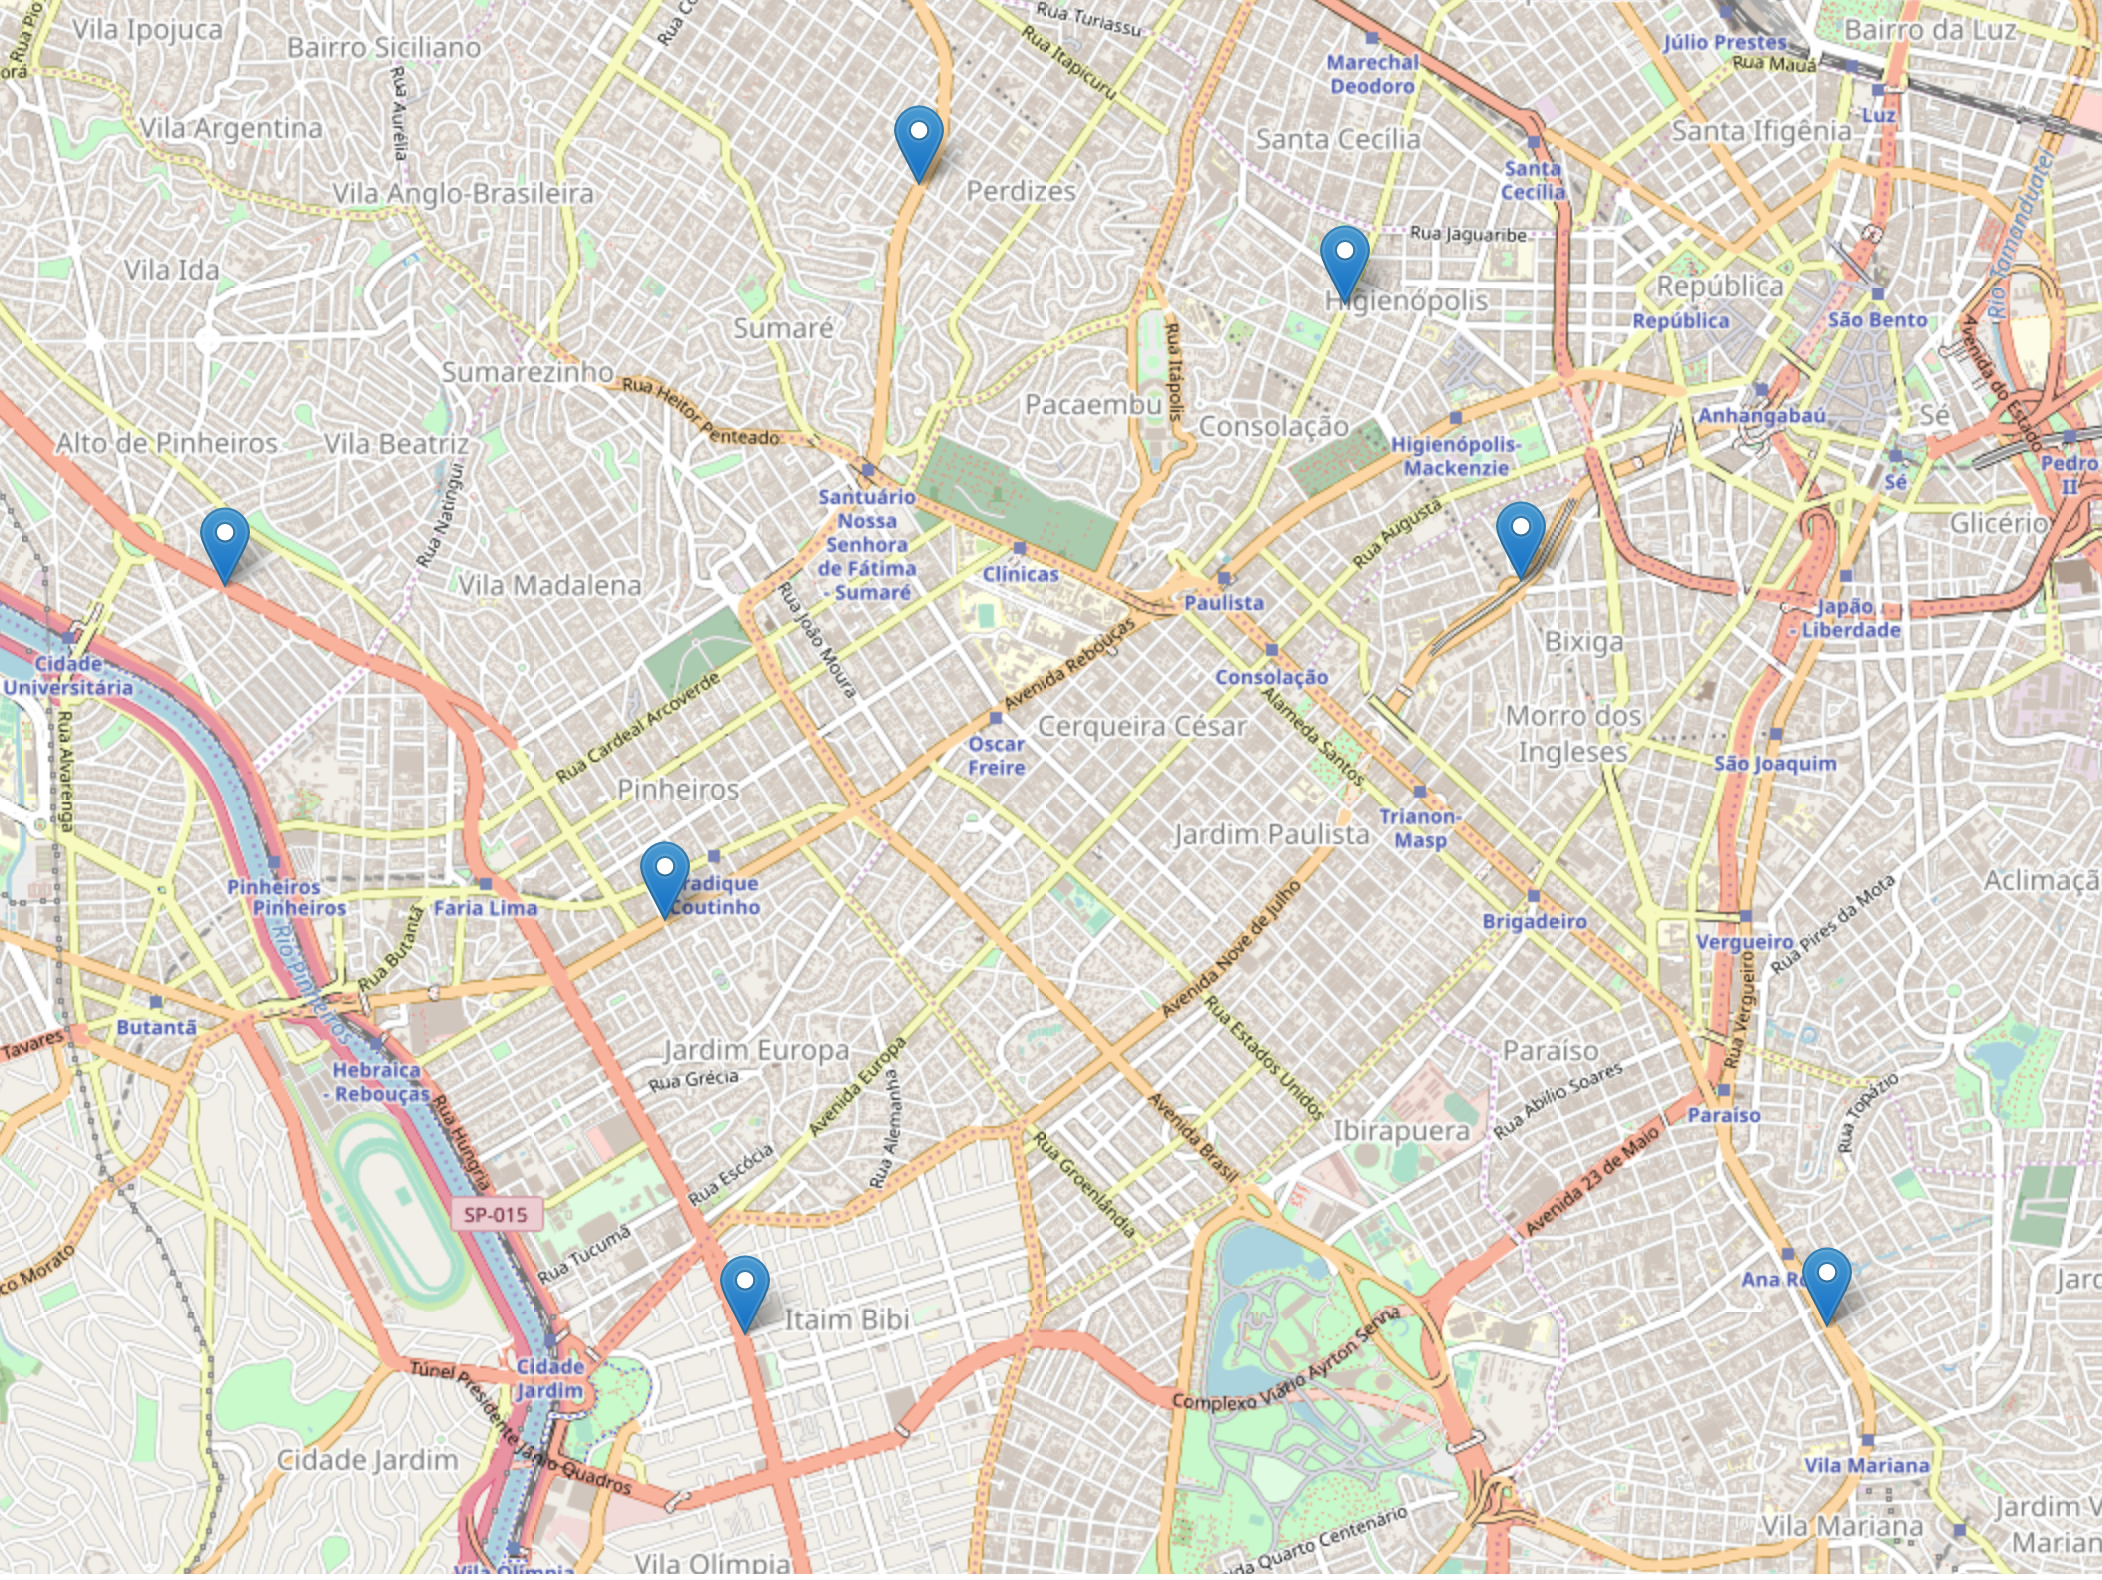
\includegraphics[width=\textwidth]{pmvs_locations.png}
            \caption{Posição das PMVs}
        \end{minipage}
        \hspace{0.5cm}
        \begin{minipage}[b]{0.45\linewidth}
            \centering
            \includegraphics[width=\textwidth]{events_edges_map.png}
            \caption{Vias fechadas}
        \end{minipage}
    \end{figure}
\end{frame}

\begin{frame}{Tráfego de Carros Inteligente}
    \begin{block}{Infraestrutura}
        \begin{itemize}
            \item 2 \textit{laptops} com:
                \begin{itemize}
                    \item 2 CPUs físicas (1.8 Ghz), 8 CPUs virtuais
                    \item 8 GB de memória RAM
                    \item Debian testing (Linux 4.15)
                \end{itemize}
            \item Um executando o InterSCSimulator e o outro a Plataforma InterSCity
        \end{itemize}
    \end{block}
\end{frame}

\begin{frame}{Tráfego de Carros Inteligente}
     \begin{figure}[ht]
        \centering
        \includegraphics[width=.7\textwidth]{duracao_filtered.png}
        \caption{Duração das viagens de carro}
    \end{figure}
\end{frame}

\section{Conclusão}

\begin{frame}{Conclusão}
    \begin{itemize}
        \item A solução apresentada viabilizou a execução de experimentos de larga escala e interativos em sistemas de Cidades Inteligentes através de simulação
        \item Integração do InterSCSimulator e da plataforma InterSCity foi realizada
            \begin{itemize}
                \item Envio/recebimento de dados de sensores
                \item Envio/recebimento de dados de atuação
            \end{itemize}
        \item Estudos de caso demostraram diversos gargalos das ferramentas em ambientes de estresse (escala de uma cidade como São Paulo)
        \item Apresentou a importância desse tipo de experimentos para sistemas de Cidades Inteligentes
    \end{itemize}
\end{frame}

\begin{frame}{Conclusão}
    \centering
    \includegraphics[width=.5\textwidth]{paper.png}
    { \tiny \url{https://www.sciencedirect.com/science/article/pii/S0167739X18307301} }
\end{frame}

\begin{frame}{Conclusão}
    \begin{block}{Limitações}
        \begin{itemize}
            \item Falta validação da solução proposta com outras ferramentas
            \item Não necessidade de implementação de módulo de tradução semântica
            \item Experimento do estudo de caso sobre Tráfego de Carros Inteligente
                \begin{itemize}
                    \item Falta de análise aprofundada das entradas da simulação
                    \item Infraestrutura com poucos recursos computacionais
                \end{itemize}
        \end{itemize}
    \end{block}
\end{frame}

\begin{frame}{Conclusão}
    \begin{block}{Trabalhos Futuros}
        \begin{itemize}
            \item Utilização de diferentes ferramentas
                \begin{itemize}
                    \item Possível necessidade de tradutor semântico
                \end{itemize}
            \item Implementação de novos cenários de Cidades Inteligentes na solução já integrada
                \begin{itemize}
                    \item Identificação de novos gargalos
                \end{itemize}
            \item Utilização de outros protocolos para realização da comunicação entres as ferramentas
        \end{itemize}
    \end{block}
\end{frame}

%\section{Introduction}
%
%\begin{frame}{Context}
%  \begin{itemize}
%    \item The copyright compromise seeked to balance public and private interests
%    \item Nowadays, changes to the law and technological advances all but destroyed this balance
%    \item[]
%    \item As a reaction, the free software movement was created
%    \begin{itemize}
%      \item Return to sharing (of source code) and to collaboration (exchange of ideas and team work)
%      \item Formalization with the GNU project
%      \item Only really possible when there are favourable conditions for source code exchange
%      \begin{itemize}
%        \item as highlighted by the growth that accompanied the Internet boom
%      \end{itemize}
%    \end{itemize}
%  \end{itemize}
%
%\end{frame}
%
%\begin{frame}[plain]
%  \includegraphics[width=\textwidth]{interscity-logo}
%\end{frame}
%
%\begin{frame}[standout]
%	This is a problem!
%\end{frame}
%
%\begin{frame}{Goals}
%  \begin{block}{Functional requirements}
%    \begin{itemize}
%      \item Integration and Management of \alert{IoT} Devices
%      \item Data Acquisition, Storing, and Processing
%      \item Context-awareness
%      \item City Resource Discovery
%      \item Geolocation-based Services
%      \item External data access
%    \end{itemize}
%  \end{block}
%\end{frame}
%
%\section{Concepts}
%
%\begin{frame}{Concepts}
%  \begin{columns}[t]
%    \col
%      \begin{coloredblock}{red!90!black}{Functional requirements}
%        \begin{itemize}
%          \item Integration and Management of IoT Devices
%          \item Data Acquisition, Storing, and Processing
%          \item Context-awareness
%          \item City Resource Discovery
%          \item Geolocation-based Services
%          \item External data access
%        \end{itemize}
%      \end{coloredblock}
%
%    \col
%      \begin{coloredblock}{red!90!black}{Non-functional requirements}
%        \begin{itemize}
%          \item Interoperability
%          \item Scalability
%          \item Security
%          \item Privacy
%          \item Evolvability
%          \item Adaptability
%        \end{itemize}
%      \end{coloredblock}
%  \end{columns}
%\end{frame}
%
%\begin{frame}{Theorems and proofs}
%  \pause
%  \begin{theorem}[An example theorem]
%    Theorem\dots
%  \end{theorem}
%
%  \pause
%  \begin{example}[An example of an example]
%    Example\dots
%  \end{example}
%
%  \pause
%  \begin{proof}[An example proof]
%    Proof\dots
%  \end{proof}
%
%  \pause
%  \begin{definition}[An example definition]
%    Definition\dots
%  \end{definition}
%
%  \pause
%  \begin{proposition}[An example proposition]
%    Proposition\dots
%  \end{proposition}
%\end{frame}
%
%\section{Related Works}
%
%\begin{frame}{Related Works}
%\end{frame}
%
%\section{Methodology}
%
%\begin{frame}{Methodology}
%\end{frame}
%
%\section{Results}
%
%\subsection{Validation and Analysis}
%
%\begin{frame}{Validation}
%\end{frame}
%
%\begin{frame}{Case Study}
%\end{frame}
%
%\section{Conclusion and Future works}
%
%\begin{frame}{Conclusion and Future works}
%\end{frame}
%
%\section{References}
%
%\begin{frame}[allowframebreaks]{References}
%  \printbibliography
%\end{frame}
%
%% Recapitulando
%\begin{frame}{\insertshorttitle}
%  \overview
%
%  % \begin{center} acrescenta espaço vertical;
%  % como possivelmente temos bem pouco espaço aqui,
%  % vamos usar centering
%  {
%    \centering\noindent%
%    \url{https://gitlab.com/link-of-your-repository}\par
%  }
%
%\end{frame}
%
%\showqrcode
%
\customtitlepage
\appendix
%
%\begin{frame}{Extra info}
%  \begin{itemize}
%    \item It is usually useful to have some extra slides addressing likely questions from the audience at the end of the presentation
%    \item By putting them after the ``appendix'' command, they are not counted in the page count indicator
%  \end{itemize}
%\end{frame}

\end{document}
